\section{Derivação Implícita}

\begin{frame}
  \begin{columns}[onlytextwidth]
    \column{0.49\textwidth}\vspace*{-0.5cm}\small
      \begin{itemize}\justifying
        \item Até agora temos trabalhado com funções \mbox{\textbf{explicitamente}} definidas, ou seja, funções da forma
        \begin{equation*}
          y = f(x),
        \end{equation*}
        na qual estabelece explicitamente a variável dependente $y$ em termos da variável independente $x$. Em outras palavras, \textbf{a variável $y$ aparece sozinha em um dos lados da equação};
        \item No entanto, algumas funções (ou curvas) são definidas através de equações que não deixam exposta a relação entre as variáveis $x$ e $y$. Em tais situações, { a variável dependente $y$ não se encontra sozinha em um dos lados da equação.}
      \end{itemize}
    \hfill
    \column{0.49\textwidth}\vspace*{-0.5cm}
      \begin{definition}[Função Implícita]\justifying
        Dizemos que uma dada equação em $x$ e $y$ define a função $f$ \textbf{implicitamente} se o \mbox{gráfico} de $y=f(x)$ coincidir com alguma porção do gráfico da equação.
      \end{definition}

      Definição alternativa\\

      \begin{definition}[Função Implícita]\justifying
          Considere a equação
          \begin{align}\label{eq:funcao-implicita}
            F(x,y)=0.
          \end{align}
          
          Dizemos que a função $y=f(x)$ é \mbox{definida} \textbf{implicitamente} pela equação \eqref{eq:funcao-implicita} se , ao substituirmos $y$ por $f(x)$ em \eqref{eq:funcao-implicita}, esta \mbox{equação} se transforma numa identidade.
      \end{definition}
  \end{columns}
\end{frame}

\begin{frame}
    \vspace{-15pt}
    \begin{columns}\justifying
        \column{.5\textwidth}
        % EXEMPLO
        \begin{example-highlight}
            A função
            \begin{equation}\label{eq:funcao-explicita-exemplo-1}
              y = \frac{x-1}{x+1}
            \end{equation}
            define $y$ explicitamente em termos de $x$. Por outro lado, a equação 
            \begin{equation*}\label{eq:funcao-implicita-exemplo-1}
              yx + y + 1 - x = 0
            \end{equation*}
            define a função em \eqref{eq:funcao-explicita-exemplo-1} implicitamente.
            
            De fato, substituindo \eqref{eq:funcao-explicita-exemplo-1} na equação $$(x + 1)y + 1 - x = 0,$$ obtemos a identidade $$(x + 1)\cdot \frac{x-1}{x+1} + 1 - x = 0.$$
        \end{example-highlight}
        \hfill
        \column{.5\textwidth}
        % EXEMPLO
        \begin{example-highlight}
            A equação $$x^2+\dfrac{1}{2}y -1 = 0$$ defini implicitamente a função $y = 2(1-x^2)$.
            
            De fato, substituindo $y = 2(1-x^2)$ na equação $x^2+\dfrac{1}{2}y -1 = 0$, obtemos a identidade
            $$x^2+\dfrac{1}{2}\cdot 2(1-x^2) -1 = 0.$$
        \end{example-highlight}
    \end{columns}
\end{frame}

\begin{frame}
    \vspace{-15pt}
    \begin{columns}\justifying
      \column{.5\textwidth}
        % EXEMPLO
        \begin{example-highlight}
            A equação $x^2 + y^2 = 4$ defini implicitamente uma infinidade de funções.
            
            De fato, resolvendo a equação para $y$ em função de $x$, vem naturalmente:
            \begin{align*}
                y = \pm\sqrt{4-x^2}.
            \end{align*}
            Os gráficos dessas funções são, respectivamente, as semi-circunferências superior e inferior da circunferência de raio $2$ (Figura).
            
            Podemos obter outras funções implícitas da equação $x^2+y^2=4$. Se tomarmos um \mbox{$c\in\mathbb{R}$} qualquer entre $-2$ e $2$, definimos a função por partes:
            \begin{align*}
                h(x)=\begin{cases}
                    \sqrt{4-x^2}, & \text{para }  x\geq c\\
                    -\sqrt{4-x^2}, & \text{para } x < c.
                \end{cases}
            \end{align*}
        \end{example-highlight}      
      \column{.5\textwidth}
      \begin{figure}
    \centering
    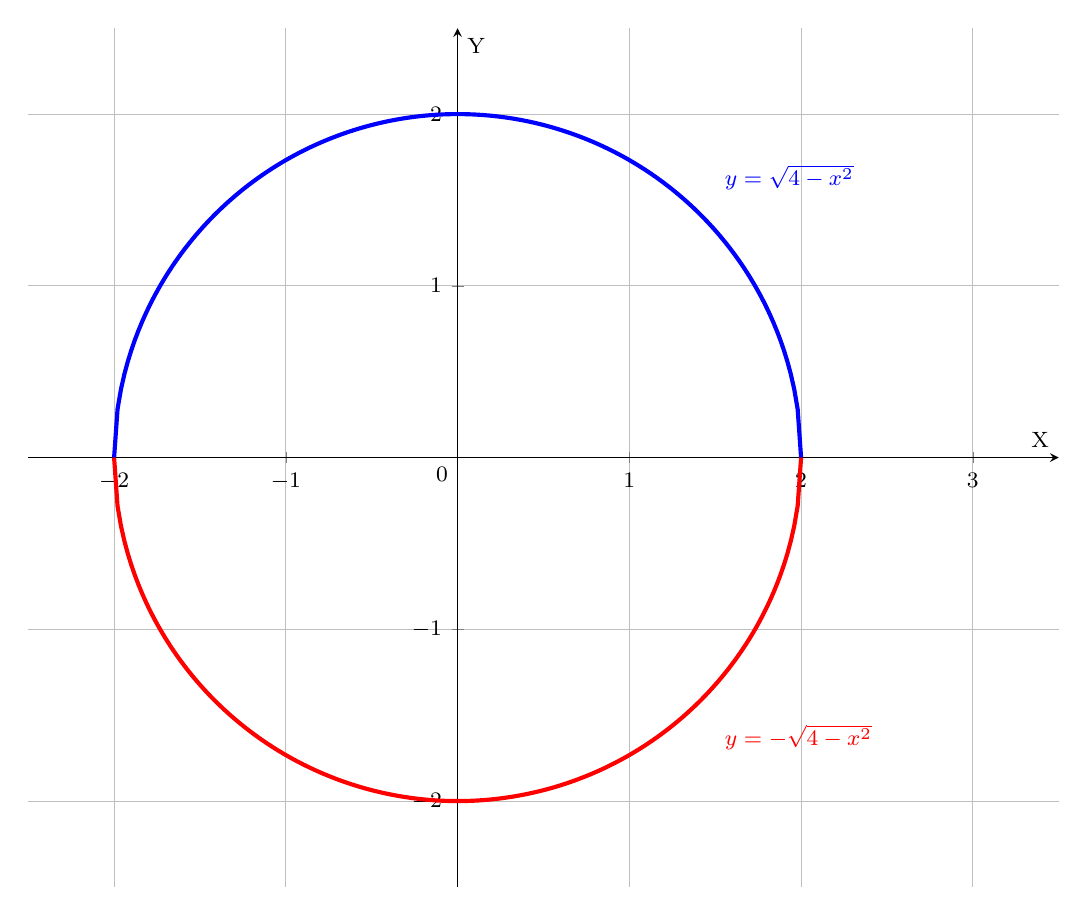
\begin{tikzpicture}
    \begin{axis}[scale=1.5,
            font=\footnotesize,
    	    width=.85\linewidth,
    		xlabel={X},ylabel={Y},
    		xtick = {-3,-2,...,3},
    		ytick = {-3,-2,...,3},
    		xmin=-2.5,xmax=3.5,
    		ymin=-2.5,ymax=2.5,
    		restrict x to domain=-2:3,
    		axis lines=center,
    		grid=both,
    		% grid style={line width=.1pt, draw=gray!10},
      %       major grid style={line width=.2pt,draw=gray!50},
      %       minor tick num=4,enlargelimits={abs=0.5},
    		% axis lines=center,
    		axis equal image,
    		]
    		
    		\node[below left] at (0,0) {$0$};
        	
        	\addplot[domain=-2:2,samples=201,
line width=1.5pt, blue]{sqrt(4-x^2)};
            \addplot[domain=-2:2,samples=201,
line width=1.5pt, red]{-sqrt(4-x^2)};

            \node[above right,blue] at (1.5,1.5) {$y=\sqrt{4-x^2}$};
            \node[below right,red] at (1.5,-1.5) {$y=-\sqrt{4-x^2}$};
    	\end{axis}    
    \end{tikzpicture}
    % \caption{Caption}
    % \label{fig:my_label}
\end{figure}
    \end{columns}
\end{frame}

% OBSERVAÇÃO
\begin{frame}
    % \begin{columns}[onlytextwidth]
    %   \column{.5\textwidth}
      \begin{alertblock}{OBSERVAÇÃO}\justifying
      Nem sempre é possível encontrar a forma explícita de uma função definida implicitamente, por exemplo, $$y^4+3xy+2\ln y = 0.$$
      
      Contudo, o método de derivação implícita permite encontrar a derivada de uma função assim definida, sem a necessidade de explicitá-la.
      \end{alertblock}
    %   \column{.5\textwidth}
    % \end{columns}
\end{frame}

\begin{frame}
  \begin{columns}[onlytextwidth]
    \begin{column}{0.49\textwidth}\vspace*{-0.5cm}
      \begin{itemize}\justifying
      
        \item Temos do exemplo anterior
        \begin{equation}\label{eq:funcao-implicita-exemplo}
          yx + y + 1 - x = 0
        \end{equation}
        define implicitamente $y$ em função de $x$.
        \item \textbf{Qual é a derivada de $y(x)$?}
        \item Dado que
        \begin{equation*}
          y = \frac{x-1}{x+1},
        \end{equation*}
        podemos usar a regra do quociente para obter a derivada desejada;
        \item Assim, temos que
        \begin{equation*}
          y^{\prime} = \frac{(x+1)\cdot 1 - (x-1)\cdot 1}{(x+1)^{2}} = \frac{2}{(x+1)^{2}}
        \end{equation*}
        \item No entanto, é possível obter o mesmo resultado sem explicitar $y$ em função de $x$;
      \end{itemize}
    \end{column}
    \begin{column}{0.49\textwidth}\vspace*{-0.5cm}
      \begin{itemize}
        \item Para isso, derivamos em relação a $x$ os dois lados da equação \eqref{eq:funcao-implicita-exemplo}
        \begin{equation*}
          \frac{d}{dx}\left[yx + y + 1 - x\right] = \frac{d}{dx}\left[0\right]
        \end{equation*}
        \item Pelas propriedades algébricas das derivadas, temos:
        \begin{equation*}
          \frac{d}{dx}\left[yx\right] + \frac{d}{dx}\left[y\right] + \frac{d}{dx}\left[1\right] - \frac{d}{dx}\left[x\right] = 0
        \end{equation*}
        \item \textbf{Supondo} que $y=f(x)$, segue:
        \begin{equation*}
          \frac{d}{dx}\left[y\right]\cdot x + y\cdot\frac{d}{dx}\left[x\right] + \frac{d}{dx}\left[y\right] - 1 = 0
        \end{equation*}
        \item Donde obtém-se:
        \begin{equation*}
          xy^{\prime} + y  + y^\prime = 1 \Rightarrow y^{\prime} = \frac{1-y}{x+1}.
        \end{equation*}
        \item Note que a derivada obtida está na forma implícita.
      \end{itemize}
    \end{column}
  \end{columns}
\end{frame}

\begin{frame}
  \begin{columns}[onlytextwidth]
    \begin{column}{0.5\textwidth}\vspace*{-0.5cm}
      \begin{example}
        Determine a reta tangente à circunferência
        \begin{equation*}
          x^{2} + y^{2} = 25
        \end{equation*}
        no ponto $P(3,\,-4)$.
      \end{example}
    \end{column}
    \begin{column}{0.5\textwidth}
      \begin{figure}
        \includefigure[width=0.9\textwidth]{exemplo1.pdf}
      \end{figure}
    \end{column}
  \end{columns}
\end{frame}

\begin{frame}
  \begin{columns}[onlytextwidth]
    \column{0.5\textwidth}\vspace*{-0.5cm}
      \begin{example}
        Dada a equação $$x^3-x^2y + y^2 + 2 = 0$$ e considerando $y=f(x)$, determine $\dfrac{dy}{dx}$.
      \end{example}
    \hfill
    \column{0.5\textwidth}
  \end{columns}
\end{frame}

% \subsection{Derivada das Potências de x}
% \begin{frame}
%   \begin{theorem}[Derivada das Potências de $x$]
%     Seja $f:I\rightarrow\mathbb{R}$ a função definida por $f(x) = x^{r}$, com $r\in\mathbb{Q}$. Então, 
%     \begin{equation*}
%       f^{\prime}(x) = r\cdot x^{r-1}.
%     \end{equation*}
%   \end{theorem}
%   \begin{columns}[onlytextwidth]
%     \begin{column}{0.55\textwidth}
%       \begin{example-highlight}
%         Determine as derivadas das funções a seguir.
%         \begin{enumerate}
%           \item $y = -\dfrac{1}{\sqrt[3]{x}}$
%           \item $f(x) = \sqrt{25-x^{2}}$
%         \end{enumerate}
%       \end{example-highlight}
%     \end{column}
%     \begin{column}{0.43\textwidth}\vspace{-0.6cm}
%     \end{column}
%   \end{columns}
% \end{frame}
